\chapter{Vari\'aci\'os elvek a fizik\'aban}
 
 \section{Mechanika}
  
  A kényszerfeltételek osztályozása (\ref{ss3:kenyszerfeletetelek}. fejezet), a Lagrange-féle első és másodfajú egyenletek (\ref{ss1:dalembert}. és \ref{ss1:lagrange2}. fejezetek), a Hamilton-elv (\ref{ss1:hamiltonelv}. fejezet).
  
 \section{Kvantummechanika}
  
  \subsection{A Rayleigh--Ritz-féle variációs elv}
   
   Definiáljuk az energia funkcionált: $E[\psi]=\frac{\bra{\psi}\opH\ket{\psi}}{\bra{\psi}\et{\psi}}$. 
   
   Állítás: ha az energia funkcionál stacioner egy $\psi$-re, akkor az a $\psi$ kielégíti a Schrödinger-egyenletet, és a hozzá tartozó energia éppen $E[\psi]$. 
   
   Bizonyítás: ha $E[\psi]$ stacioner egy adott $\psi$-re, akkor az e szerinti variációja eltűnik. Variáljunk $\bra{\psi}$ szerint:
   \al{
    0&=\delta_{\bra{\psi}}E[\psi]
      =
       \frac{\bra{\delta\psi}\opH\ket{\psi}}{\bra{\psi}\et{\psi}}-\frac{\bra{\psi}\opH\ket{\psi}}{\bra{\psi}\et{\psi}^2}\bra{\delta\psi}\et{\psi}
      =\frac{1}{\bra{\psi}\et{\psi}}\cdot\left(\bra{\delta\psi}\opH\ket{\psi}-\frac{\bra{\psi}\opH\ket{\psi}}{\bra{\psi}\et{\psi}}\bra{\delta\psi}\et{\psi}\right)\\
     &=\frac{1}{\bra{\psi}\et{\psi}}\cdot\bigg\langle\delta\psi\bigg|\left(\opH-\frac{\bra{\psi}\opH\ket{\psi}}{\bra{\psi}\et{\psi}}\right)\bigg|\psi\bigg\rangle
      =\frac{1}{\bra{\psi}\et{\psi}}\cdot\big\langle\delta\psi\big|\left(\opH-E[\psi]\right)\big|\psi\big\rangle,
   }
   ez pedig akkor teljesül minden $\bra{\delta\psi}$-re, ha 
   \al{
    \opH\ket{\psi}=E[\psi]\ket{\psi}.
   }
   
   Ezt az eredményt úgy is megkaphatjuk, ha a $\bra{\psi}\opH\ket{\psi}$ mennyiséget variáljuk azzal a mellékfeltétellel, hogy $\bra{\psi}\et{\psi}=1$. Bevezetve az $E$ Lagrange-multiplikátort:
   \al{
    0=\delta_{\bra{\psi}}\Big(\bra{\psi}\opH\ket{\psi}-E\big(\bra{\psi}\et{\psi}-1\big)\Big)
     =\bra{\delta\psi}\opH\ket{\psi}-E\bra{\delta\psi}\et{\psi}
     =\bra{\delta\psi}\Big(\opH\ket{\psi}-E\ket{\psi}\Big).
   }
   
   \paragraph{Ritz-féle variációs elv}
    
    Az $E[\psi]$ tetszőleges $\psi$-re legalább akkora, mint az alapállapoti energia. A bizonyításhoz felhasználjuk, hogy $\opH$ hermitikus, így létezik teljes ortonormált bázist alkotó sajátfüggvény-rendszere. Ezen a bázison kifejthetőek a $\psi$ állapotok: $\psi=\suml{i}{}a_i\psi_i$. Ha ezt behelyettesítjük az energiafunkcionálba:
    \al{
     E[\psi]
      =\frac{\suml{i}{}\abs{a_i}^2E_i}{\suml{i}{}\abs{a_i}^2}
      \underbrace{\geq}_{E_0=\min\limits_{i}E_i}
       \frac{\suml{i}{}\abs{a_i}^2E_0}{\suml{i}{}\abs{a_i}^2}
       =E_0.
    }
    Az egyenlőség akkor áll fenn, ha $\psi=\psi_0$ azaz az alapállapoti hullámfüggvényt helyettesítjük a funkcionálba. A bizonyításhoz felhasználtuk, hogy a $\opH$ operátor alulról korlátos, így sajátértékei között van minimális. Relativisztikus esetben ez nem igaz, így ott nem ezt a variációs módszert használni. 
    
    Az alapállapot megkeresése úgy lehetséges, hogy készítünk egy próbafüggvényt, melyben több paraméter van, ezzel elkészítjük az energia funkcionált, majd ennek a függvénynek keressük meg a minimumát. Így tehát azt az egyenletrendszert kell megoldani, hogy $\pder{E\big[\psi(a_1,a_2,\dots)\big]}{a_i}=0$, $\forall$ $i$-re. 
    
  \subsection{Harmonikus oszcillátor alapállapota variációs módszerrel}
   
   A Hamilton-operátor: $\opH=\frac{\opp^2}{2m}+\frac{1}{2}m\omega^2\opx^2=-\frac{\hbar^2}{2m}\Delta+\frac{1}{2}m\omega^2 x^2$.
   
   {\bf 1. közelítés} Keressük az alapállapoti megoldást a következő alakban: 
   \eq{
    \psi(x)=\begin{cases}
             \big(x^2-a^2\big)^2 &\abs{x}<a\\
             0&\abs{x}>a
            \end{cases}.
   }
   Behelyettesítve:
   \al{
    \bra{\psi}\opH\ket{\psi}
     &=\intl{-\infty}{\infty}\dd x\,\psi^*(x)\left(-\frac{\hbar^2}{2m}\Delta+\frac{1}{2}m\omega^2 x^2\right)\psi(x)\\
     &=\intl{-a}{a}\dd x\,\big(x^2-a^2\big)^2\left(-\frac{\hbar^2}{2m}\Delta+\frac{1}{2}m\omega^2 x^2\right)\big(x^2-a^2\big)^2\\
     &=\intl{-a}{a}\dd x\,\Big(x^4-2x^2a^2+a^4\Big)\left(-\frac{\hbar^2}{2m}\Big(12x^2-4a^2\Big)+\frac{1}{2}m\omega^2 x^2\Big(x^4-2x^2a^2+a^4\Big)\right)\\
     &=\intl{-a}{a}\dd x\,\bigg[
       \left(\frac{2\hbar^2 a^6}{m}\right)
      +\left(\frac{1}{2} m \omega ^2 a^8 -\frac{10 \hbar^2 a^4}{m}\right)x^2
      +\left(\frac{14 \hbar^2  a^2}{m} -2 m \omega ^2 a^6 \right)x^4+\\
     &\qquad\qquad
      +\left(3 m \omega ^2 a^4 -\frac{6 \hbar^2}{m} \right)x^6
      +\left(-2 m\omega^2 a^2 \right)x^8
      +\left(\frac{1}{2} m\omega ^2\right)x^{10}\bigg]\\
     &=\frac{128 a^{11} m \omega ^2}{3465}+\frac{128 a^7 \hbar^2}{105 m},\\
    \bra{\psi}\et{\psi}
     &=\intl{-\infty}{\infty}\dd x\,\psi^*(x)\psi(x)
      =\intl{-\infty}{\infty}\dd x\,\big(x^2-a^2\big)^4\\
     &=\intl{-\infty}{\infty}\dd x\,\Big(a^8-4 a^6 x^2+6 a^4 x^4-4 a^2 x^6+x^8\Big)
      =\frac{256 a^9}{315},\\
    E\big[\psi(x)\big]
     &=\frac{\frac{128 a^{11} m \omega ^2}{3465}+\frac{128}{105} a^7 \hbar^2 m}{\frac{256 a^9}{315}}
      =\frac{3 \hbar^2 }{2 a^2 m}+\frac{1}{22} a^2 m \omega ^2.
   }
   
   Az energia funkcionál szélsőértéket vesz fel, ha
   \al{
    0
     &=\pder{E\big[\psi(x)\big]}{a}
      =-\frac{3 \hbar^2 }{ a^3 m}+\frac{1}{11} a m \omega ^2
     &\Rightarrow
     &&a^2=\sqrt{33}\frac{\hbar}{m\omega}
   }
   \al{
    E\left[\psi\left(a^2=\sqrt{33}\frac{\hbar}{m\omega}\right)\right]
     &=\frac{3 \hbar^2 }{2 m}\cdot\frac{m\omega}{\sqrt{33}\hbar} +\frac{1}{22} \sqrt{33}\frac{\hbar}{m\omega} m \omega ^2 
      =\frac{\hbar\omega}{2}\cdot\sqrt{\frac{12}{11}}.
   }
   
   {\bf 2. közelítés} Most keressük a megoldást Gauss-függvényként:
   \al{
    \psi(x)=e^{-a\frac{x^2}{2}}.
   }
   Elkészítjük az előző integrálokat ezzel a függvénnyel is:
   \al{
    \bra{\psi}\opH\ket{\psi}
     &=\intl{-\infty}{\infty}\dd x\,e^{-a\frac{x^2}{2}}\left(-\frac{\hbar^2}{2m}\Delta+\frac{1}{2}m\omega^2 x^2\right)e^{-a\frac{x^2}{2}}\\
     &=\intl{-\infty}{\infty}\dd x\,e^{-a\frac{x^2}{2}}\left(-\frac{\hbar^2}{2m}\Big(a^2 x^2 e^{-a\frac{x^2}{2}}-a e^{-a\frac{ x^2}{2}}\Big)+\frac{1}{2}m\omega^2 x^2e^{-a\frac{x^2}{2}}\right)\\
     &=\intl{-\infty}{\infty}\dd x\,\left[\left(-\frac{\hbar^2a^2}{2m}+\frac{1}{2}m\omega^2\right) x^2 e^{-a x^2}+\frac{\hbar^2 a}{2m}e^{-a x^2}\right].
   }
   Használjuk, hogy $\intl{-\infty}{\infty}\dd x\,e^{-ax^2}=\sqrt{\frac{\pi}{a}}$, illetve hogy $\intl{-\infty}{\infty}\dd x\,x^2e^{-ax^2}=\frac{1}{2a}\sqrt{\frac{\pi}{a}}$,
   \al{
    \bra{\psi}\opH\ket{\psi}
     &=\left(-\frac{\hbar^2a^2}{2m}+\frac{1}{2}m\omega^2\right)\frac{1}{2a}\sqrt{\frac{\pi}{a}} + \frac{\hbar^2 a}{2m}\sqrt{\frac{\pi}{a}}
      =\frac{m\omega^2}{4a}\sqrt{\frac{\pi}{a}} + \frac{\hbar^2 a}{4m}\sqrt{\frac{\pi}{a}},\\
    \bra{\psi}\et{\psi}
     &=\intl{-\infty}{\infty}\dd x\,e^{-ax^2}=\sqrt{\frac{\pi}{a}},\\
    E\big[\psi(x)\big]
     =\frac{m\omega^2}{4a} + \frac{\hbar^2 a}{4m}.
   }
   Ennek minimuma:
   \al{
    0
     &=\pder{E\big[\psi(x)\big]}{a}
      =-\frac{m\omega^2}{4a^2} + \frac{\hbar^2}{4m}.
     &\Rightarrow
     &&a=\frac{m\omega}{\hbar}
   }
   \al{
    E\left[\psi\left(a=\frac{m\omega}{\hbar}\right)\right]
     &=\frac{m\omega^2}{4}{\frac{\hbar}{m\omega}} + \frac{\hbar^2 }{4m}{\frac{m\omega}{\hbar}}
      =\frac{\hbar\omega}{2}.
   }
   
  \subsection{Hidrogén-atom alapállapota variációs módszerrel}
   
   A Schrödinger-egyenlet gömbi koordináta-rendszerben:
   \al{
    \opH=-\frac{\hbar^2}{2m}
    \left[
     \frac{1}{r^2}\pder{}{r}\left(r^2 \pder{}{r}\right)
     +\frac{1}{r^2}\left(\frac{1}{\sin\vartheta}\pder{}{\vartheta}\left(\sin\vartheta\pder{}{\vartheta}\right)+\frac{1}{\sin^2\varphi}\pder{^2}{\varphi^2}\right)
    \right]+V(\rv).
   }
   A próbafüggvény legyen gömbszimmetrikus:
   \al{
    \psi(r)=A e^{-\frac{r}{r_0}}.
   }
   Behelyettesítve:
   \al{
    \bra{\psi}\opH\ket{\psi}
     &=\intl{0}{\infty}\dd x\,A e^{-\frac{r}{r_0}}
      \left(
       -\frac{\hbar^2}{2m}
     \frac{1}{r^2}\pder{}{r}\left(r^2 \pder{}{r}\right)-\frac{1}{4\pi\ep_0}\frac{e^2}{r}
      \right)
      A e^{-\frac{r}{r_0}}\\
     &=\intl{0}{\infty}\dd x\,\left[
       -\frac{\hbar^2}{2m} \left(\frac{A^2 e^{-\frac{2r}{r_0}}}{r_0^2}-\frac{2 A^2 e^{-\frac{2r}{r_0}}}{rr_0}\right)
       -\frac{1}{4\pi\ep_0}\frac{e^2}{r}A^2 e^{-\frac{2r}{r_0}}\right]
      \\
     &=\intl{0}{\infty}\dd x\,\left[
       -\frac{\hbar^2}{2mr_0^2} A^2 e^{-\frac{2r}{r_0}}
       +\frac{\hbar^2A^2}{mr_0}\frac{1}{r} e^{-\frac{2r}{r_0}}
       -\frac{1}{4\pi\ep_0}\frac{e^2}{r}A^2 e^{-\frac{2r}{r_0}}\right]
      \\
     &=A^2\intl{0}{\infty}\dd x\,\left[
       -\frac{\hbar^2}{2mr_0^2} e^{-\frac{2r}{r_0}}
       +\left(\frac{\hbar^2}{mr_0}-\frac{e^2}{4\pi\ep_0}\right)\frac{1}{r} e^{-\frac{2r}{r_0}}
       \right].
   }
   A második tag divergens. Ezt úgy tudjuk kiküszöbölni, ha $r_0$-at úgy választjuk, hogy a második tag eltűnjön. Emiatt: $r_0=\frac{4\pi\ep_0\hbar^2}{me^2}$. Az integrál, mivel $\intl{0}{\infty}\dd x\,e^{-\frac{2r}{r_0}}=\frac{r_0}{2}$, így
   \al{
    \bra{\psi}\opH\ket{\psi}
     &=-A^2\frac{\hbar^2}{2mr_0^2}\frac{r_0}{2}\\
    \bra{\psi}\et{\psi}
     &=\intl{0}{\infty}\dd x\,A^2 e^{-2\frac{r}{r_0}}=A^2\frac{r_0}{2}\\
    E[\psi]
     &=-\frac{\hbar^2}{2mr_0^2}
      =-\frac{\hbar^2}{2m}\frac{m^2e^4}{16\pi^2\ep_0^2\hbar^4}
      =-\frac{me^4}{32\pi^2\ep_0^2\hbar^2}
      =-\frac{m e^4 k^2}{2\hbar^2}.
   }
   
  \subsection{Hartree-közelítés}\label{ss:10-Hartree}
   
   A zárt héjú kötött elektronrendszer problémáját szeretnénk megoldani. A Hartree-közelítés lényege, hogy a megoldást az egyrészecske hullámfüggvények szorzataként írjuk fel, és ezzel az próbafüggvénnyel végezzük el a variációt. A Hamilton-operátor:
   \al{
    \opH=-\suml{i=1}{N}\frac{\hbar^2}{2m}\Delta_i-\frac{Ze^2}{4\pi\ep_0}\suml{i=1}{N}\frac{1}{r_i}+\frac{e^2}{4\pi\ep_0}\suml{\mv{i,j}}{}\frac{1}{\abs{r_i-r_j}}=\suml{i=1}{N}\opH_i+\suml{\mv{i,j}}{}\opV_{i,j},
   }
   a hullámfüggvény pedig 
   \al{
    \psi(\rv_1,\rv_2,\dots\rv_N)=\phi_1(\rv_1)\phi_2(\rv_2)\cdot\cdots\cdot\phi_N(\rv_N)
   }
   ahol $\phi_i$-k az egyrészecske hullámfüggvények. Az egyrészecske állapotok ortonormált bázist alkotnak, így $\bra{\phi_i}\et{\phi_j}=\delta_{ij}$.
   
   Az energia funkcionál, figyelembevéve a normáltsági feltételt:
   \al{
    \tilde{E}_\text{H}[\psi]
     &=\left[\prodl{i=1}{N}\bra{\phi_i}\right]\left[\suml{i=1}{N}\opH_i+\suml{\mv{i,j}}{}\opV_{i,j}-\suml{i=1}{N}\ep_i\big(\bra{\phi_i}\et{\phi_i}-1\big)\right]\left[\prodl{i=1}{N}\ket{\phi_i}\right]\\
     &=\suml{i=1}{N}\bra{\phi_i}\opH_i\ket{\phi_i}+\suml{\mv{i,j}}{}\bra{\phi_i}\bra{\phi_j}\opV_{i,j}\ket{\phi_j}\ket{\phi_i}-\suml{i=1}{N}\ep_i\big(\bra{\phi_i}\et{\phi_i}-1\big).
   }
   Ennek a variálása $\bra{\phi_k}$ szerint:
   \al{
    \delta_{\bra{\phi_k}}\tilde{E}_\text{H}[\psi]
     &=\opH_k\ket{\phi_k}+\suml{\substack{i=1\\i\ne k}}{N}\bra{\phi_i}\opV_{i,k}\ket{\phi_i}\ket{\phi_k}-\ep_k\ket{\phi_k}=0,
   }
   így
   \aln{
    &\left(\opH_k+\opV_k\right)\ket{\phi_k}=\ep_k\ket{\phi_k}
    &\opV_k=\suml{\substack{i=1\\i\ne k}}{N}\bra{\phi_i}\opV_{i,k}\ket{\phi_i}.\label{eq:10-hartree}
   }
   A kölcsönhatás kiírva:
   \al{
    V_k(\rv_k)
     =\frac{e^2}{4\pi\ep_0}\intl{V}{}\drh\suml{\substack{i=1\\i\ne k}}{N}\abs{\phi_i(\rv_i)}^2\frac{1}{\abs{\rv_i-\rv_k}}.
   }
   Láthatjuk tehát, hogy a megoldandó egyenlet szétesett egyrészecske egyenletekké, azonban minden egyenlet esetében a potenciál tartalmazza a többi egyenlet megoldásaként kapott egyrészecske hullámfüggvényeket. Emiatt az egyenletek csak együtt oldhatóak meg iterációs módszerrel. Valamilyen kezdeti hullámfüggvényekből kiindulva felépítjük a potenciálokat, majd megoldjuk az egyenleteket. Ezek után a megoldásokkal elkészítjük az új potenciálokat, és újra megoldjuk az egyenletet. Ezt ismételjük, amíg a módszer nem konvergál: ez a ``selfconsistent field method''.
   
   Az állapot energiáját kifejezhetjük az $\ep_i$ Lagrange-multiplikátorokkal. \Eqaref{eq:10-hartree} egyenlet alapján:
   \al{
    \bra{\phi_k}\ep_k\ket{\phi_k}
     &=\ep_k
      =\bra{\phi_k}\opH_k\ket{\phi_k}+\bra{\phi_k}\opV_k\ket{\phi_k}
      =\bra{\phi_k}\opH_k\ket{\phi_k}+\suml{\substack{i=1\\i\ne k}}{N}\bra{\phi_k}\bra{\phi_i}\opV_{i,k}\ket{\phi_i}\ket{\phi_k}.
   }
   Ennek az összege minden $k$-ra:
   \al{
    \suml{k=1}{N}\ep_k
     &=\suml{k=1}{N}\bra{\phi_k}\opH_k\ket{\phi_k}+\suml{\substack{i=1,k=1\\i\ne k}}{N}\bra{\phi_k}\bra{\phi_i}\opV_{i,k}\ket{\phi_i}\ket{\phi_k}\\
     &=\suml{k=1}{N}\bra{\phi_k}\opH_k\ket{\phi_k}+2\suml{\mv{i,k}}{N}\bra{\phi_k}\bra{\phi_i}\opV_{i,k}\ket{\phi_i}\ket{\phi_k}
      =E_\text{H}[\psi]+\suml{\mv{i,k}}{N}\bra{\phi_k}\bra{\phi_i}\opV_{i,k}\ket{\phi_i}\ket{\phi_k}
   }
   \aln{
    E_\text{H}[\psi]=\suml{k=1}{N}\ep_k-\suml{\mv{i,k}}{N}\bra{\phi_k}\bra{\phi_i}\opV_{i,k}\ket{\phi_i}\ket{\phi_k}.\label{eq:10-hartreeE}
   }
   
   Ez a módszer nem veszi figyelembe, hogy az elektronállapotok teljesen antiszimmetrikusak. Ha azt is figyelembe szeretnénk venni, akkor nem használhatjuk a fenti próbafüggvényt.
   
   A Hartree--Fock-módszerben a hullámfüggvényt antiszimmetrizáljuk, a próbafüggvények ott Sla\-ter-de\-ter\-mi\-nán\-sok, azaz az egyrészecske hullámfüggvények teljesen antiszimmetrikus kombinációjából állnak. Ekkor az energia:
   \al{
    E_\text{HF}[\psi]=E_\text{H}[\psi]-\suml{\mv{i,k}}{N}\bra{\phi_k}\bra{\phi_i}\opV_{i,k}\ket{\phi_k}\ket{\phi_i}.
   } 
   
 \section{Elektrodinamika -- Elektromos és mágneses terek anyag jelenlétében}
  
  Sztatikus elektromos és mágneses jelenségek anyagban illetve a határfeltételek: \ref{ss1:elsztat}. és \ref{ss1:magnetosztatika}. fejezet. 
  
  \subsection{Frekvenciafüggő dielektromos állandó}
   
   A polarizáció egy időfüggő elektromos tér ($\Ev(t,\rv)$) hatására:
   \al{
    \Pv(\rv,t)=\intl{-\infty}{\infty}\dd t'\theta(t-t')\mat{G}(t,t')\Ev(t',\rv),
   }
   ahol figyelembe vettük, hogy csak a múlt lehet hatással a jelen pillanatban lévő polarizációra. Tekintsünk izotrop anyagot, ahol minden egy irányba mutat, illetve tegyük fel, hogy nincs kitüntetett időpont: $G(t,t')=G(t-t')$. Ekkor a szuszceptibilitás, mint a külső térre adott válaszfüggvény:
   \al{
    &\ep_0\chi(t-t')=\theta(t-t')G(t,t')
    &P(t)=\intl{-\infty}{\infty}\dd t'\ep_0\chi(t-t')E(t').
   }
   Ezt Fourier-transzformálva:
   \al{
    P(\omega)=\ep_0\chi(\omega)E(\omega),
   }
   vagyis
   \al{
    D(\omega)&=\ep_0 E(\omega)+P(\omega)=\ep_0 E(\omega)+\ep_0\chi(\omega)E(\omega)
     =\ep_0\big(1+\chi(\omega)\big)E(\omega)\\
    \ep_r(\omega)&=1+\chi(\omega).
   }
   Mivel a fizikai mennyiségek valósak, ezért $\chi^*(\omega)=\chi(-\omega)$. 
   
   Oldjuk meg a fenti problémát egy modellre. Tekintsünk harmonikus potenciálban mozgó csillapított töltést, mint az anyag építőkövét. Ennek a mozgásegyenlete:
   \al{
    &m\partial_t^2x(t)+\gamma\partial_t x(t)+\omega_0^2 x(t)=qE(t)
    &\Rightarrow
    &&-\omega^2 m qx(\omega)-i\omega\gamma q x(\omega)+\omega_0^2 qx(\omega)=q^2E(\omega),
   } 
   ahol $qx(\omega)$ a polarizáció éppen, így $p(\omega)=\frac{q^2}{m}\frac{E(\omega)}{\omega_0^2-i\gamma\omega-\omega^2}$. A makroszkópikus polarizációs sűrűség ennek az $n$-szerese, ahol $n$ a töltéssűrűség. Több sajátfrekvenciát feltételezve:
   \al{
    &P(\omega)=\suml{i}{}\frac{n_iq_i^2}{m_i}\frac{E(\omega)}{\omega_{i,0}^2-i\gamma\omega-\omega^2}
    &\ep_r(\omega)=1+\suml{i}{}\frac{n_iq_i^2}{\ep_0m_i}\frac{1}{\omega_{i,0}^2-i\gamma\omega-\omega^2}
   }
   
   $\ep_r(\omega)$ ismeretében megadható a törésmutató: $n(\omega)=\sqrt{\ep_r(\omega)}$, mellyel: $k(\omega)=\frac{\omega}{c_r(\omega)}=\frac{\omega}{c}n_\text{r}(\omega)$. Így egy monokromatikus hullám terjedése:
   \al{
    E(t,\rv)=E_0 e^{-i\omega t+i\frac{\omega}{c}n_\text{r}(\omega)\cdot \frac{\kv}{k}\rv}.
   }
   Ha $\gamma\neq 0$ akkor $n_t(\omega)$-nak van képzetes része is: 
   \al{
    \Im{\ep_\text{r}(\omega)}
     =\suml{i}{}\frac{n_iq_i^2}{\ep_0m_i}\Im\left[\frac{1}{\omega_{i,0}^2-i\gamma\omega-\omega^2}\right]
     =\suml{i}{}\frac{n_iq_i^2}{\ep_0m_i}\frac{\gamma\omega}{\big(\omega_{i,0}^2-\omega^2\big)^2 +\gamma^2\omega^2}> 0,
   }
   így a hullám csillapodik:
   \al{
    E(t,\rv)=E_0 e^{-i\omega t+i\frac{\omega}{c}\Re\big[n_\text{r}(\omega)\big]\cdot \frac{\kv}{k}\rv}\cdot e^{-\frac{\omega}{c}\Im\big[n_\text{r}(\omega)\big]\cdot \frac{\kv}{k}\rv},
   }
   ahol $\Im[n_\text{r}(\omega)]$ az abszorpciós együttható. 
   
   Szabad elektrongázra, ahol $\omega_{i,0}=0$ és $\gamma=0$:
   \al{
    &\ep_r(\omega)
     =1-\frac{nq^2}{\ep_0m}\frac{1}{\omega^2}
     =1-\frac{\omega_\text{P}^2}{\omega^2}
    &\omega_\text{P}^2=\frac{nq^2}{\ep_0m}.
   }
   \begin{itemize}
    \item $\omega<\omega_\text{P}$: $\ep_r(\omega)<0$ $\Rightarrow$ $n_\text{r}(\omega)$ tisztán képzetes, vagyis az elektrongáz nem átlátszó.
    \item $\omega>\omega_\text{P}$: $\ep_r(\omega)>0$ $\Rightarrow$ $0<n_\text{r}(\omega)<1$ tisztán valós, vagyis az elektrongáz tökéletesen átlátszó. A fázissebesség:
     \al{
      v_\text{f}=\frac{\omega}{k}=\frac{c}{n_\text{r}(\omega)}>c,
     }
     illetve a csoportsebesség:
     \al{
      v_\text{cs}=\pder{\omega}{k}=\frac{c}{n_\text{r}(\omega)+\omega\pder{n_\text{r}}{\omega}}=\frac{c}{n_\text{r}(\omega)+\omega\frac{\omega_\text{P}^2}{n_\text{r}\omega^3}}=\frac{n_\text{r}c}{n_\text{r}^2+\frac{\omega_\text{P}^2}{\omega^2}}=nc<c.
     }
    \item $\omega=\omega_\text{P}$: $\ep_r(\omega)=0$ $\Rightarrow$ $n_\text{r}(\omega)=0$. Ekkor a közegben a fázissebesség végtelen a csoportsebesség pedig nulla. 
   \end{itemize}
   
  \subsection{Homogén térbe helyezett dielektrikum/mágnesezhető gömb}
   
   A két probléma matematikailag ugyanaz, hiszen forrásmentes esetben a statikában az Maxwell-egyenletek szimmetrikusak. Megoldjuk a problémát a dielektrikumra vonatkozóan, majd átírjuk az eredményt a mágneses esetre is. 
   
   Legyen a gömb sugara $R$ relatív permittivitása pedig $\ep_\text{g}$. A külső közegben legyen a tér $\Ev_0=(0,0,E_0)$, és ennek permittivitása legyen $\ep_\text{k}$. A potenciálra a Laplace-egyenletet kell megoldani mindkét térrészben, illetve a határon illeszteni kell a két megoldást. Az egyenletek és a határfeltételek:
   \al{
    &\Delta\phi_\text{g}(\rv)=0
    &\Delta\phi_\text{k}(\rv)=0
    &&\begin{cases}
       \phi_\text{g}(r\to 0)=\text{véges}&\\
       \phi_\text{k}(r\to \infty)=-E_0r\cos\vartheta&\\
       \phi_\text{k}(r=R)=\phi_h(r=R)\\
       \ep_\text{k}\left.\pder{\phi_\text{k}}{r}\right|_{r=R}=\ep_\text{g}\left.\pder{\phi_\text{g}}{r}\right|_{r=R}&
      \end{cases}
   }
   A megoldás hengerszimmetrikus. A gömbi Laplace-egyenlet általános megoldásaival felírva:
   \al{
    &\phi_\text{k}(r,\vartheta)=\suml{l}{}\big(A_lr^l+B_lr^{-l-1}\big)P_l(\cos\vartheta),
    &\phi_\text{g}(r,\vartheta)=\suml{l}{}\big(C_lr^l+D_lr^{-l-1}\big)P_l(\cos\vartheta).
   }
   A határfeltételek alapján:
   \al{
    &\phi_\text{k}(r\to\infty,\vartheta)=-E_0r\cos\vartheta
    &\Rightarrow
    &&A_l=\begin{cases}
           -E_0&l=1\\
           0&l\ne 1
          \end{cases}.
   }
   Feltehetjük, hogy $B_l=C_l=D_l=0$, ha $l\ne 1$. A többi határfeltétel:
   \al{
    &\phi_\text{g}(r\to 0,\vartheta)=\big(C_1r+D_1r^{-2}\big)\cos\vartheta=\text{véges}
    &\Rightarrow
    &&D_1= 0\\
    &\left.
     \begin{array}{r}
      \displaystyle C_1R=-E_0R+\frac{B_1}{R^2}\\
      \displaystyle \ep_\text{k}\cdot\left(-E_0-2\frac{B_1}{R^3}\right)=\ep_r C_1
     \end{array}
     \right\}
    &\Rightarrow
    &&
    \left\{
     \begin{array}{l}
      \displaystyle B_1=\frac{\ep_\text{g}-\ep_\text{k}}{\ep_\text{g}+2\ep_\text{k}}E_0R^3\\
      \displaystyle C_1=-\frac{3\ep_\text{k}}{\ep_\text{g}+2\ep_\text{k}}E_0
     \end{array}
     \right.
   }
   Vagyis
   \al{
    &\phi_\text{k}(\rv)=-\left(1-\frac{\ep_\text{g}-\ep_\text{k}}{\ep_\text{g}+2\ep_\text{k}}\frac{R^3}{r^3}\right)\Ev_0\rv
    &\phi_\text{g}(\rv)=-\left(\frac{3\ep_\text{k}}{\ep_\text{g}+2\ep_\text{k}}\right)\Ev_0\rv.
   }
   
   Belül a tér homogén, kint pedig a tér egy homogén és egy dipól terének az összege. A dipól erőssége $\left(\phi_\text{dipól}=\frac{1}{4\pi\ep}\frac{\pv\rv}{r^3}\right)$:
   \al{
    \Pv=4\pi\ep_0\ep_\text{k}\frac{\ep_\text{g}-\ep_\text{k}}{\ep_\text{g}+2\ep_\text{k}}R^3\Ev_0.
   }
   Belül a térerősség homogén, illetve a térerősség többlet, ami létrejött ($\Ev_\text{polar}$):
   \al{
    &\Ev_\text{g}=\left(\frac{3\ep_\text{k}}{\ep_\text{g}+2\ep_\text{k}}\right)\Ev_0
    &\Rightarrow
    &&\Ev_\text{polar}=\Ev_\text{g}-\Ev_0=\frac{\ep_\text{k}-\ep_\text{g}}{\ep_\text{g}+2\ep_\text{k}}\Ev_0.
   }
   
   \paragraph{Diszkusszió} 
   \begin{itemize}
    \item $\ep_\text{k}=1$, $\ep_\text{g}=\infty$: először tekintsünk egy speciális esetet, legyen a közeg vákuum és az anyag fém. Ekkor $\pv=4\pi\ep_0R^3\Ev_0$, $\Ev_\text{g}=0$, $\Ev_\text{polar}=-\Ev_0$. 
    \item $\ep_\text{k}<\ep_\text{g}$. Ekkor $\pv \parallel \Ev_0$, vagyis a gömb úgy polarizálódik, hogy belül csökken a térerősség.
    \item $\ep_\text{k}>\ep_\text{g}$. Ekkor $\pv \parallel -\Ev_0$, így belül nő a térerősség.
   \end{itemize}
   
   \begin{figure}[ht!]
    \centering
    \subfloat[$\Ev(\rv)$ ($\ep_\text{k}<\ep_\text{g}$), $\Hv(\rv)$ ($\mu_\text{k}<\mu_\text{g}$)\label{fig:10-1}]{\begin{overpic}[width= 0.3\textwidth]{./A10tetel/Db}
      \put(0,0){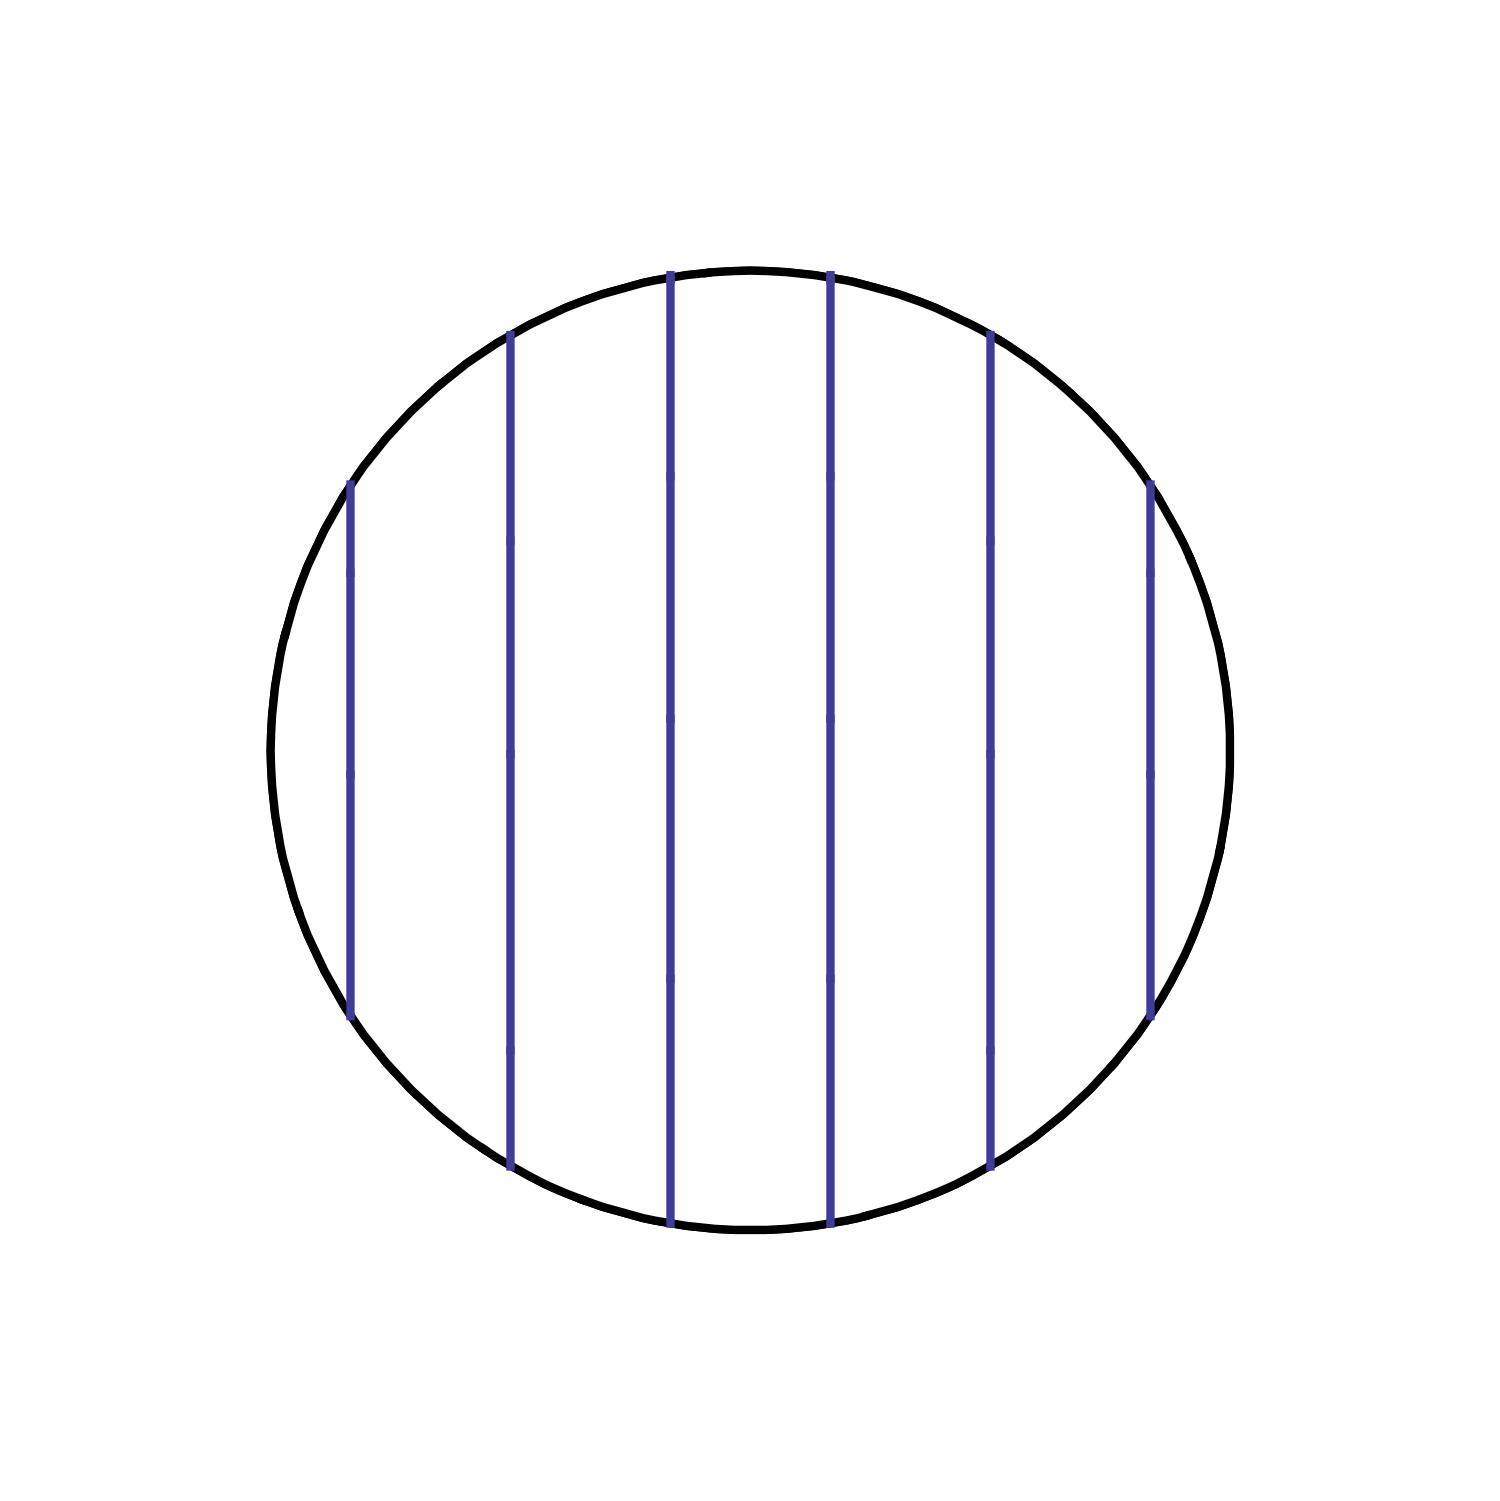
\includegraphics[width= 0.3\textwidth]{./A10tetel/Eb}}
      \put(8.4,71){\tikz \draw[-latex,thick,blue] (0,0) -- (0,0.1);}
      \put(32.8,71){\tikz \draw[-latex,thick,blue] (0,0) -- (0,0.1);}
      \put(47.8,71){\tikz \draw[-latex,thick,blue] (0,0) -- (0,0.1);}
      \put(62.6,71){\tikz \draw[-latex,thick,blue] (0,0) -- (0,0.1);}
      \put(77.5,71){\tikz \draw[-latex,thick,blue] (0,0) -- (0,0.1);}
      \put(93.0,71){\tikz \draw[-latex,thick,blue] (0,0) -- (0,0.1);}
      \put(107.6,71){\tikz \draw[-latex,thick,blue] (0,0) -- (0,0.1);}
      \put(131.8,71){\tikz \draw[-latex,thick,blue] (0,0) -- (0,0.1);}
     \end{overpic}}
    \hspace{6pt}
    \subfloat[$\Dv(\rv)$ ($\ep_\text{k}<\ep_\text{g}$, $\Bv(\rv)$ ($\mu_\text{k}<\mu_\text{g}$))\label{fig:10-2}]{\begin{overpic}[width= 0.3\textwidth]{./A10tetel/Db}
      \put(8.4,71){\tikz \draw[-latex,thick,blue] (0,0) -- (0,0.1);}
      \put(27.7,71){\tikz \draw[-latex,thick,blue] (0,0) -- (0,0.1);}
      \put(37.8,71){\tikz \draw[-latex,thick,blue] (0,0) -- (0,0.1);}
      \put(48.2,71){\tikz \draw[-latex,thick,blue] (0,0) -- (0,0.1);}
      \put(58.8,71){\tikz \draw[-latex,thick,blue] (0,0) -- (0,0.1);}
      \put(70.2,71){\tikz \draw[-latex,thick,blue] (0,0) -- (0,0.1);}
      \put(81.5,71){\tikz \draw[-latex,thick,blue] (0,0) -- (0,0.1);}
      \put(92.2,71){\tikz \draw[-latex,thick,blue] (0,0) -- (0,0.1);}
      \put(102.7,71){\tikz \draw[-latex,thick,blue] (0,0) -- (0,0.1);}
      \put(112.7,71){\tikz \draw[-latex,thick,blue] (0,0) -- (0,0.1);}
      \put(131.8,71){\tikz \draw[-latex,thick,blue] (0,0) -- (0,0.1);}
     \end{overpic}}
    \hspace{6pt}
    \subfloat[$\Ev_\text{dipól}(\rv)$ ($\ep_\text{k}<\ep_\text{g}$), $\Hv_\text{dipól}(\rv)$ ($\mu_\text{k}<\mu_\text{g}$)\label{fig:10-3}]{\begin{overpic}[width= 0.3\textwidth]{./A10tetel/Pk}
      \put(3.4,68){\tikz \draw[latex-,thick,blue] (0,0) -- (0,0.1);}
      \put(35.3,68){\tikz \draw[latex-,thick,blue] (0,0) -- (0,0.1);}
      \put(52.9,68){\tikz \draw[latex-,thick,blue] (0,0) -- (0,0.1);}
      \put(70.4,68){\tikz \draw[latex-,thick,blue] (0,0) -- (0,0.1);}
      \put(88,68){\tikz \draw[latex-,thick,blue] (0,0) -- (0,0.1);}
      \put(105.2,68){\tikz \draw[latex-,thick,blue] (0,0) -- (0,0.1);}
      \put(137,68){\tikz \draw[latex-,thick,blue] (0,0) -- (0,0.1);}      \put(60,106.3){\tikz\node[red] at (0,0) {\tiny $\pmb{\oplus}$};}
      \put(68,106.3){\tikz\node[red] at (0,0) {\tiny $\pmb{\oplus}$};}
      \put(89,98){\tikz\node[red] at (0,0) {\tiny $\pmb{\oplus}$};}
      \put(39,98){\tikz\node[red] at (0,0) {\tiny $\pmb{\oplus}$};}
      \put(60,21.7){\tikz\node[blue] at (0,0) {\tiny $\pmb{\ominus}$};}
      \put(68,21.7){\tikz\node[blue] at (0,0) {\tiny $\pmb{\ominus}$};}
      \put(89,30){\tikz\node[blue] at (0,0) {\tiny $\pmb{\ominus}$};}
      \put(39,30){\tikz\node[blue] at (0,0) {\tiny $\pmb{\ominus}$};}
     \end{overpic}}
     %
     \\
     %
     \subfloat[$\Ev(\rv)$ ($\ep_\text{k}>\ep_\text{g}$), $\Hv(\rv)$ ($\mu_\text{k}>\mu_\text{g}$)\label{fig:10-4}]{\begin{overpic}[width= 0.3\textwidth]{./A10tetel/Dk}
      \put(0,0){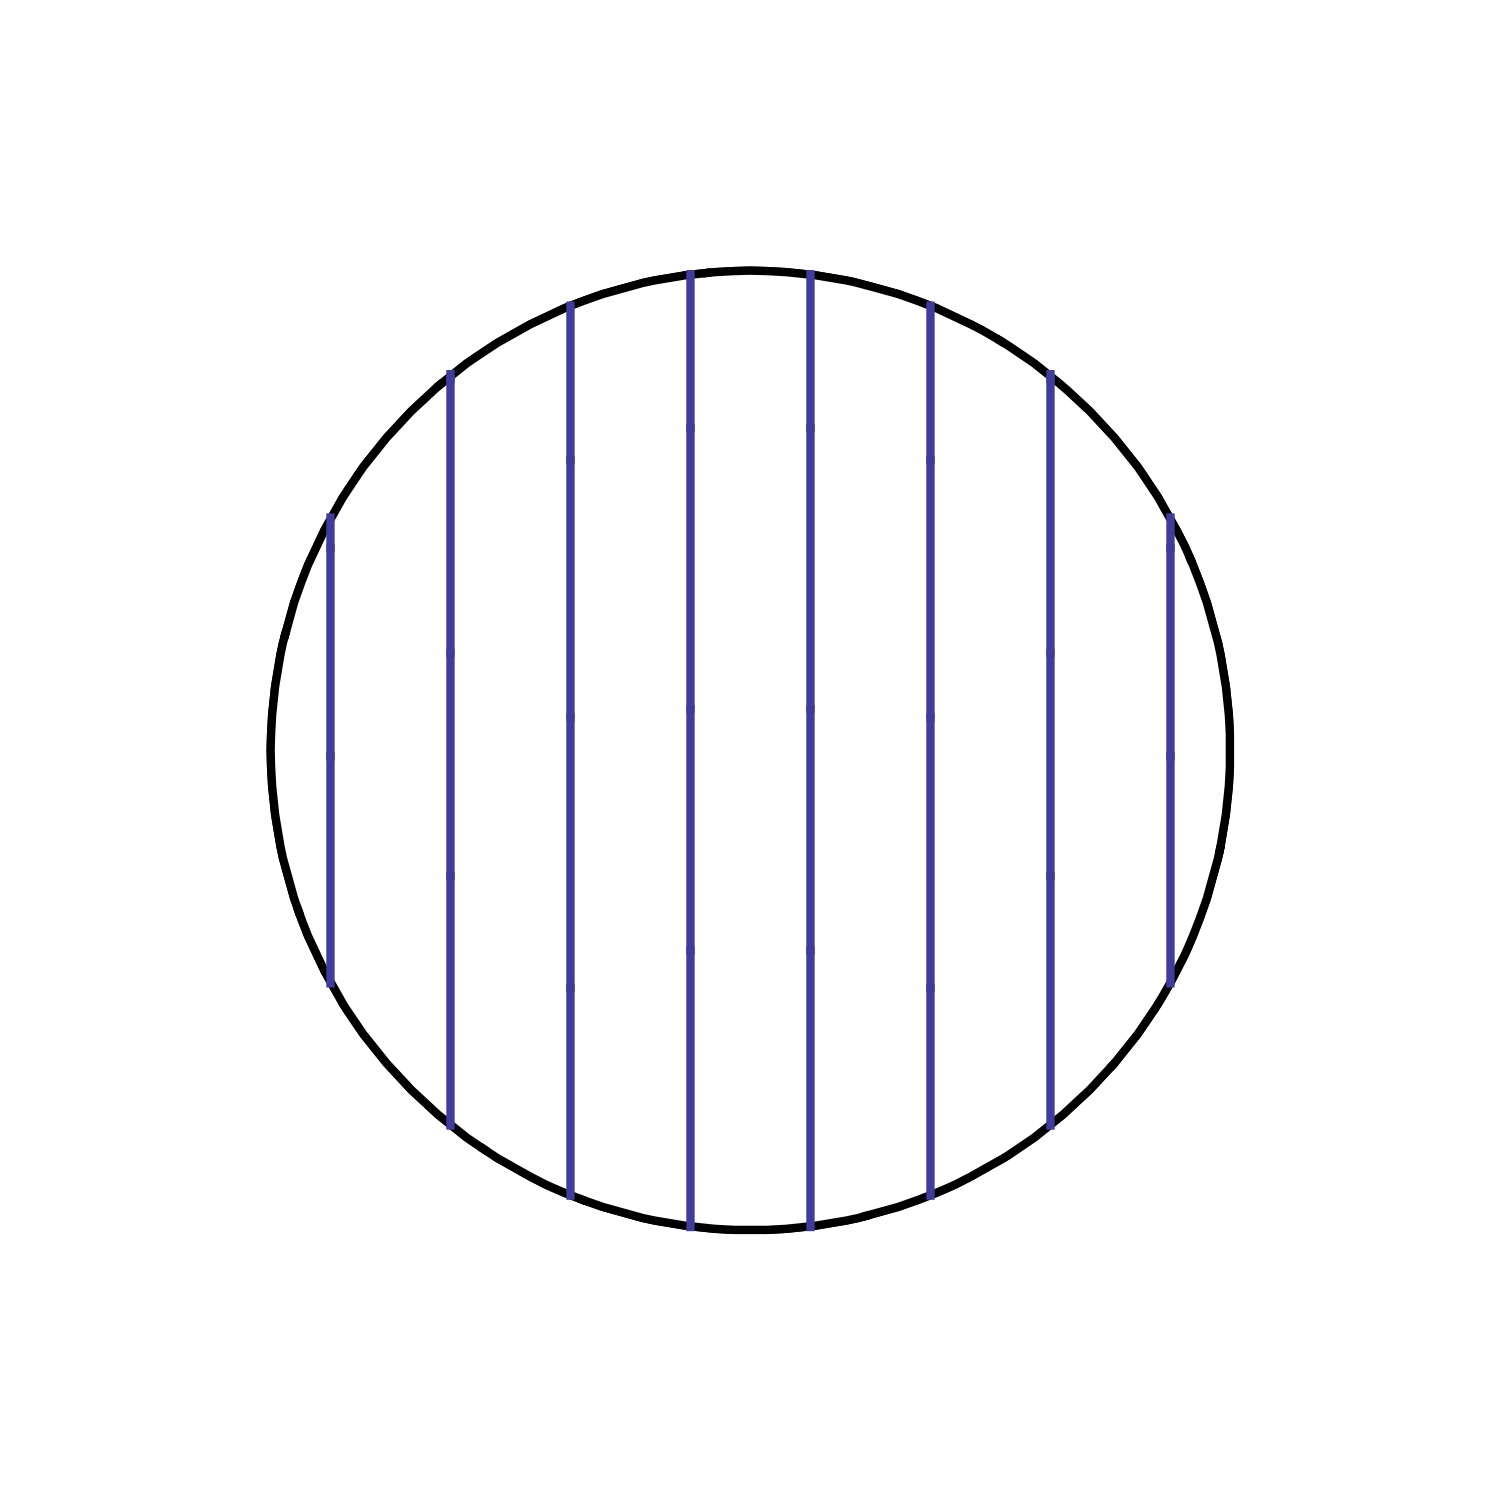
\includegraphics[width= 0.3\textwidth]{./A10tetel/Ek}}
      \put(10.5,71){\tikz \draw[-latex,thick,blue] (0,0) -- (0,0.1);}
      \put(20,71){\tikz \draw[-latex,thick,blue] (0,0) -- (0,0.1);}
      \put(30.7,71){\tikz \draw[-latex,thick,blue] (0,0) -- (0,0.1);}
      \put(42,71){\tikz \draw[-latex,thick,blue] (0,0) -- (0,0.1);}
      \put(53.2,71){\tikz \draw[-latex,thick,blue] (0,0) -- (0,0.1);}
      \put(64.4,71){\tikz \draw[-latex,thick,blue] (0,0) -- (0,0.1);}
      \put(75.9,71){\tikz \draw[-latex,thick,blue] (0,0) -- (0,0.1);}
      \put(87,71){\tikz \draw[-latex,thick,blue] (0,0) -- (0,0.1);}
      \put(98.4,71){\tikz \draw[-latex,thick,blue] (0,0) -- (0,0.1);}
      \put(109.6,71){\tikz \draw[-latex,thick,blue] (0,0) -- (0,0.1);}
      \put(120.2,71){\tikz \draw[-latex,thick,blue] (0,0) -- (0,0.1);}
      \put(130,71){\tikz \draw[-latex,thick,blue] (0,0) -- (0,0.1);}
     \end{overpic}}
    \hspace{6pt}
    \subfloat[$\Dv(\rv)$ ($\ep_\text{k}>\ep_\text{g}$), $\Bv(\rv)$ ($\mu_\text{k}>\mu_\text{g}$)\label{fig:10-5}]{\begin{overpic}[width= 0.3\textwidth]{./A10tetel/Dk}
      \put(10.5,71){\tikz \draw[-latex,thick,blue] (0,0) -- (0,0.1);}
      \put(20,71){\tikz \draw[-latex,thick,blue] (0,0) -- (0,0.1);}
      \put(31.7,71){\tikz \draw[-latex,thick,blue] (0,0) -- (0,0.1);}
      \put(51.2,71){\tikz \draw[-latex,thick,blue] (0,0) -- (0,0.1);}
      \put(70.2,71){\tikz \draw[-latex,thick,blue] (0,0) -- (0,0.1);}
      \put(89.2,71){\tikz \draw[-latex,thick,blue] (0,0) -- (0,0.1);}
      \put(108.5,71){\tikz \draw[-latex,thick,blue] (0,0) -- (0,0.1);}
      \put(120.2,71){\tikz \draw[-latex,thick,blue] (0,0) -- (0,0.1);}
      \put(130,71){\tikz \draw[-latex,thick,blue] (0,0) -- (0,0.1);}
     \end{overpic}}
    \hspace{6pt}
    \subfloat[$\Ev_\text{dipól}(\rv)$ ($\ep_\text{k}>\ep_\text{g}$), $\Hv_\text{dipól}(\rv)$ ($\mu_\text{k}>\mu_\text{g}$)\label{fig:10-6}]{\begin{overpic}[width= 0.3\textwidth]{./A10tetel/Pk}
      \put(3.4,71){\tikz \draw[-latex,thick,blue] (0,0) -- (0,0.1);}
      \put(35.3,71){\tikz \draw[-latex,thick,blue] (0,0) -- (0,0.1);}
      \put(52.9,71){\tikz \draw[-latex,thick,blue] (0,0) -- (0,0.1);}
      \put(70.4,71){\tikz \draw[-latex,thick,blue] (0,0) -- (0,0.1);}
      \put(88,71){\tikz \draw[-latex,thick,blue] (0,0) -- (0,0.1);}
      \put(105.2,71){\tikz \draw[-latex,thick,blue] (0,0) -- (0,0.1);}
      \put(137,71){\tikz \draw[-latex,thick,blue] (0,0) -- (0,0.1);}
      \put(60,106.3){\tikz\node[blue] at (0,0) {\tiny $\pmb{\ominus}$};}
      \put(68,106.3){\tikz\node[blue] at (0,0) {\tiny $\pmb{\ominus}$};}
      \put(89,98){\tikz\node[blue] at (0,0) {\tiny $\pmb{\ominus}$};}
      \put(39,98){\tikz\node[blue] at (0,0) {\tiny $\pmb{\ominus}$};}
      \put(60,21.7){\tikz\node[red] at (0,0) {\tiny $\pmb{\oplus}$};}
      \put(68,21.7){\tikz\node[red] at (0,0) {\tiny $\pmb{\oplus}$};}
      \put(89,30){\tikz\node[red] at (0,0) {\tiny $\pmb{\oplus}$};}
      \put(39,30){\tikz\node[red] at (0,0) {\tiny $\pmb{\oplus}$};}
     \end{overpic}}
    \caption{A homogén gömb körüli elektromos térerősség, eltolás és polarizációs tér, ha $\ep_\text{k}<\ep_\text{g}$ (első sor), illetve ha $\ep_\text{k}>\ep_\text{g}$ (második sor). Mivel $\Dv$ forrása a szabad töltések, ezért az itt folytonos. $\Ev$ forrása bármilyen töltés, és itt van felületi töltéssűrűség, ezért vannak olyan $\Ev$ vonalak, amelyek a felületen keletkeznek/végződnek.}
    \end{figure}
   
   Térjünk át a mágneses esetre. Az analógia: $\Ev\leftrightarrow\Hv$, $\Dv\leftrightarrow\Bv$, $\ep_\text{r}\leftrightarrow\mu_\text{r}$ és $\phi\leftrightarrow\phi_\text{M}$. Így
   \al{
    &\phi_\text{M,k}(\rv)=-\left(1-\frac{\mu_\text{g}-\mu_\text{k}}{\mu_\text{g}+2\mu_\text{k}}\frac{R^3}{r^3}\right)\Hv_0\rv
    &\phi_\text{M,g}(\rv)=-\left(\frac{3\mu_\text{k}}{\mu_\text{g}+2\mu_\text{k}}\right)\Hv_0\rv.
   }
   Az indukált mágneses dipól erőssége:
   \al{
    \emv=4\pi\frac{\mu_\text{g}-\mu_\text{k}}{\mu_\text{g}+2\mu_\text{k}}R^3\Hv_0.
   }
   Belül a mágneses tér 
   \al{
    &\Hv_\text{g}=\left(\frac{3\mu_\text{k}}{\mu_\text{g}+2\mu_\text{k}}\right)\Hv_0
    &\Rightarrow
    &&\Bv_\text{g}=\left(\frac{3\mu_\text{k}}{\mu_\text{g}+2\mu_\text{k}}\right)\frac{\mu_\text{g}}{\mu_\text{k}}\mu_0\Hv_0
    &&\Mv=\frac{\emv}{V}=3\frac{\mu_\text{g}-\mu_\text{k}}{\mu_\text{g}+2\mu_\text{k}}\Hv_0.
   }
   
%    Itt a külső anyagot vákuumnak vesszük: $\mu_\text{k}=1$. 
   \begin{itemize}
    \item $\mu_\text{g}>\mu_\text{k}$, paramágneses eset: ez felel meg az ábrák közül az első sornak. Speciális eset a ferromágneses eset, amikor $\mu_\text{g}\gg\mu_\text{k}=1$. Ekkor a belső tér $\Hv_\text{g}\approx0$, vagyis az indukálódott momentum teljesen leárnyékolja a külső teret. Az indukció: $\Bv_\text{g}=\mu_0\frac{3}{2}\Hv_0$.
    \item $\mu_\text{g}<\mu_\text{k}$, diamágneses eset: ez pedig az ábrák második sorának fele meg. Speciális eset az ideális diamágneses eset, amikor $\chi=-1$. Ekkor $\Hv_\text{g}=\frac{3}{2}\Hv_0$ és $\Bv_\text{g}=0$. Itt $\Hv$ nem értelmezhető a gömb belsejében.
   \end{itemize}
   
   
   
  
  